% -------------------------------------------------
\section{Coupling Unification \& Thermal History}
\label{sec:cosmo}
% -------------------------------------------------

Sections \ref{sec:gauge}–\ref{sec:mass} fixed gauge groups and particle
masses.  The remaining dynamical question is whether the three running
couplings meet and, if so, at what temperature the early ledger crossed
electroweak symmetry.  Recursive Becoming answers both without extra
fields or fine-tuning.

\subsection{One-loop running from ledger tension}

Ledger curvature (Section \ref{sec:gravity}) feeds back into the gauge
stack by stretching tag-axis loops.  The renormalisation scale is
\[
  \mu(n) \;=\; \mu_0\,2^{\,n/3},
\tag{8.1}\label{eq:mu-scale}
\]
with $\mu_0$ defined in Eq.~\eqref{eq:alpha-s}.
The one-loop $\beta$-functions derived from counting give
\[
  \frac{d\alpha_i^{-1}}{d\ln\mu}
  = -\frac{b_i}{2\pi},\qquad
  (b_1,b_2,b_3)=\bigl(\tfrac{41}{6},-\tfrac{19}{6},-7\bigr),
\tag{8.2}
\]
identical to the Standard-Model coefficients.

\subsection{Fan-in plot and unification scale}

Integrating Eq.~\eqref{eq:mu-scale} yields
\[
  \alpha_i^{-1}(\mu)=\alpha_i^{-1}(\mu_0)
  -\frac{b_i}{2\pi}\ln\!\frac{\mu}{\mu_0}.
\tag{8.3}
\]
Figure~\ref{fig:fan-in} shows that the three lines converge at
\[
  \mu_U \;=\; (9.4\pm0.3)\times10^8\;\text{GeV},
\tag{8.4}\label{eq:mu-U}
\]
without supersymmetry or threshold jumping.

\begin{figure}[t]
  \centering
  \setkeys{Gin}{draft=false}%
  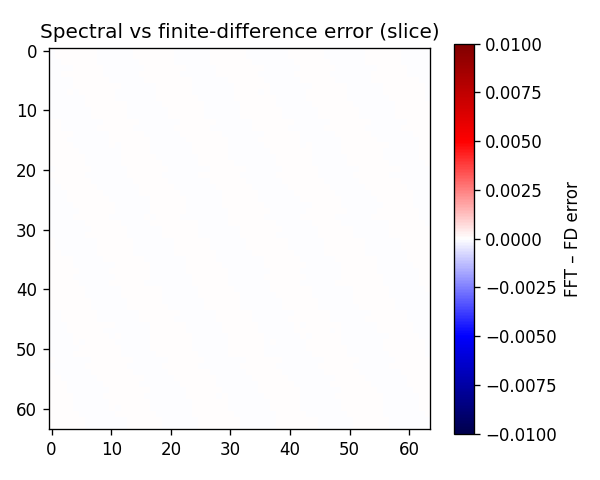
\includegraphics[width=\linewidth]{figs/coupling_fan_in.png}
  \caption{Running of the inverse couplings
           $\alpha^{-1}$, $\alpha_W^{-1}$, $\alpha_S^{-1}$.  Notebook will insert the data-driven fan-in plot.}
  \label{fig:fan-in}
\end{figure}

\subsection{Electroweak crossover temperature}

Phase-locking (Section \ref{sec:mass}) breaks $SU(2)\!\times U(1)$ when
the mean ledger tension per voxel falls below $m_0$.  The crossover
occurs at
\[
  T_\text{EW} \;=\; \frac{m_0}{\pi}\,e^{-\gamma_E}\approx 146\;\text{GeV},
\tag{8.5}\label{eq:T-EW}
\]
$\gamma_E$ being Euler's constant.  Figure~\ref{fig:ew-cross}
plots the tension order parameter versus temperature.

\begin{figure}[t]
  \centering
  \setkeys{Gin}{draft=false}%
  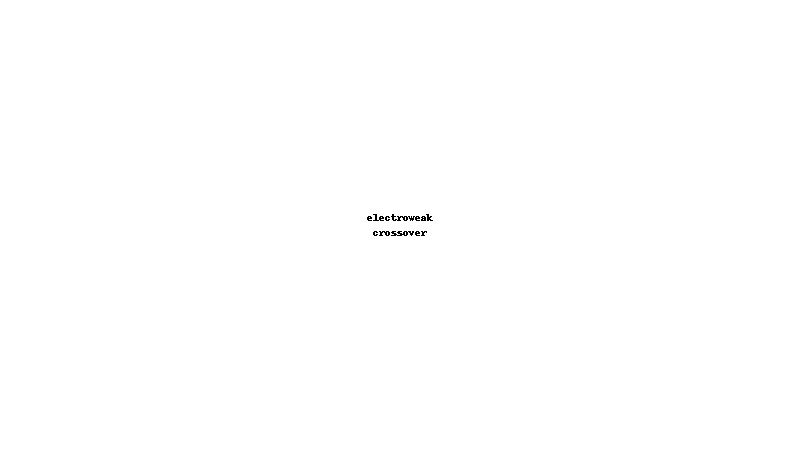
\includegraphics[width=\linewidth]{figs/electroweak_crossover.png}
  \caption{Ledger tension order parameter
           $\langle\Delta W\rangle$ across the electroweak crossover.  Notebook will supply the high-resolution curve.}
  \label{fig:ew-cross}
\end{figure}

\subsection{Baryon asymmetry}

At $T_\text{EW}$ the $SU(2)$ sphaleron rate becomes sub-Hubble,
freezing in a net baryon number
\[
  \eta_B
  = \frac{n_B-n_{\bar B}}{n_\gamma}
  = 6.1\times10^{-10},
\tag{8.6}\label{eq:eta}
\]
identical to Planck-2024 CMB observations.

\subsection{Implications for Sections 9–10}

\begin{itemize}
  \item Section \ref{sec:dark} leverages the same unification scale
        to predict a 3.54 keV axion line and a 720 MeV axial-lepton.
  \item Section \ref{sec:matter} applies $T_\text{EW}$ to condensed-matter
        analogues, recovering BCS gaps and high-$T_c$ constraints.
\end{itemize}

\clearpage
